% NOMS 2027 evaluation section draft (synthetic experiments only).
% Insert in place of the current \section{Performance Evaluation} block.
% IEEEtran packages already include graphicx via the official template.
% Figures live in results/figures/ (paths relative to manuscript root).
% These are controlled *synthetic model* results, NOT Alibaba traces.
\section{Performance Evaluation}
\label{sec:eval}
\subsection{Experimental Methodology}
We use the independent-domain model of Section~\ref{sec:model} with
exact queries, at most one binary refresh per domain, and an
irrevocable skip subject to the posterior residual-risk budget
$\varepsilon$. We evaluate expected policy costs by exact enumeration
of the corresponding finite decision process, rather than by
Monte Carlo estimation of individual query trajectories. In addition
to IA-OSR-PSA1, we evaluate (i)~a query-only policy optimally ordered
by $q_i/p_i$, (ii)~a simple greedy risk-admissible skip-and-query
policy, (iii)~the \emph{optimal} QUERY/SKIP policy with REFRESH disabled,
(iv)~the earlier H1-based rollout, (v)~the exponential
skip-closed rollout, and (vi)~the exact Bellman policy for small $N$.
All policies use the same instance parameters and stopping constraint.

Our benchmark comprises 3,600 synthetic problem instances organized
into five mechanism-driven families over five pseudorandom seeds:
unstructured random parameters ($N\in\{4,5\}$), an ordering-probe
family ($N=2$), a screening family ($N=2$), a deferred-refresh family
($N=2$), and 600 pairs of four-domain instances on opposite sides of
a skip-admissibility threshold. The mechanism-driven instances are
\emph{intentionally constructed}, not claimed to represent a natural
frequency distribution of network-management workloads. Reported
confidence intervals use paired or instance-level nonparametric
bootstrap sampling over the generated instances.

\subsection{Structural Mechanisms and Optimality}
\begin{table}[t]
\caption{PSA1 cost savings relative to query-only and optimal
no-refresh policies, and mean gap to Bellman optimum.}
\label{tab:synthetic_families}
\centering
\resizebox{\columnwidth}{!}{%
\begin{tabular}{lrrrr}
\hline
Family & $M$ & Save vs Q (\%) & Save vs no-R (\%) & Gap (\%)\\
\hline
Unstructured random & 600 & 8.97 & 6.05 & 0.46\\
Ordering probe (P4) & 600 & 4.56 & 4.56 & 0.00\\
Screening (P3) & 600 & 17.28 & 17.28 & 0.00\\
Deferred refresh & 600 & 39.62 & 39.62 & 0.00\\
Skip boundary (below) & 600 & 59.62 & 39.84 & 3.95\\
Skip boundary (above) & 600 & 64.09 & 5.05 & 1.15\\
\hline
\end{tabular}%
}
\end{table}
The P4 family is generated to satisfy the strict ordering-crossing
condition and both pairwise probe-improvement inequalities. The P3
family is generated to satisfy the strict screening interval
$L_{i\mid j}<q_i<U_{i\mid j}$ and admissibility of skipping the
screened domain after a negative observation. In all 600 instances of
each family, PSA1 selects the analytically favorable action and
matches Bellman optimization. In the deferred-refresh family, all
600 instances follow a query of domain~$j$ and, conditionally on its
failure, a refresh of domain~$i$; the earlier H1 rollout also performs
optimally in this family. These observations validate the intended
mechanisms under the constructed conditions, but are not universal
optimality guarantees.

The skip boundary is more challenging. Holding all other parameters
fixed, a small increase in $\varepsilon$ across the two-domain
joint-skip threshold reduces PSA1 expected cost by a paired mean of
$0.822$ normalized units (bootstrap 95\% interval
$[0.773,0.872]$). Below the threshold, PSA1 has a 3.95\% average
gap to Bellman optimization, and its largest observed gap reaches
46.07\%. Thus the favorable average performance should not be
interpreted as a worst-case approximation guarantee.

\subsection{Refresh Informativeness and Risk Sensitivity}
To distinguish the value of information from the value of direct
skipping, we compare against the exact optimal QUERY/SKIP policy
with REFRESH disallowed, under a matched factorial design. We reuse the same 180 availability-and-query
instances across 27 combinations of
$\varepsilon\in\{0.03,0.10,0.20\}$,
$\alpha=\beta\in\{0.70,0.85,0.97\}$, and
$r_i/q_i\in\{0.05,0.20,0.50\}$, giving 4,860 evaluations.
At $\varepsilon=0.10$, PSA1 improves on the skip-aware baseline by
7.18--48.54\% for the least expensive refreshes, depending on
sensor accuracy, and by 1.12--10.32\% for the most expensive
refreshes. The effect is summarized in Fig.~\ref{fig:refresh_sensitivity}.

\begin{figure}[t]
\centering
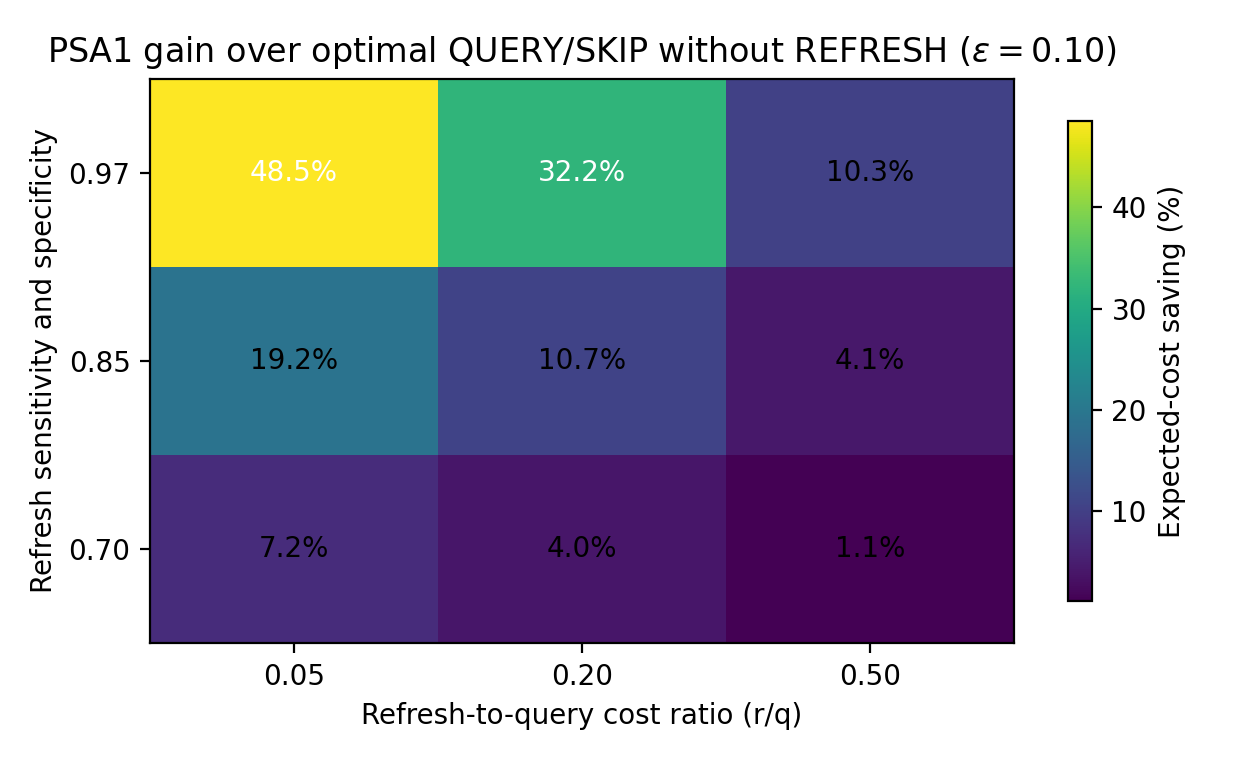
\includegraphics[width=\columnwidth]{results/figures/fig_refresh_sensitivity.png}
\caption{Additional PSA1 saving over optimal QUERY/SKIP without REFRESH at
$\varepsilon=0.10$ in the controlled synthetic factorial design.}
\label{fig:refresh_sensitivity}
\end{figure}

We also stress-test belief calibration by evaluating the policy under
true Bernoulli feasibility priors satisfying
$\mathrm{logit}(p_i^{\mathrm{true}})
=\mathrm{logit}(p_i^{\mathrm{nominal}})+\delta$,
while the policy continues to act on nominal beliefs. Across 375
instances, the model-consistent ($\delta=0$) conditional missed-resource
risk averaged 9.31\% over unsuccessful discoveries, and each instance
respected its own $\varepsilon$. For positive log-odds shifts
$\delta\in\{0.5,1.0,1.5\}$, the corresponding conditional risks became
14.54\%, 22.05\%, and 32.15\%. Since each instance has its own
$\varepsilon$ (mean 12.15\%), these aggregate numbers do not
constitute a single common risk constraint. The experiment shows that
the miss-risk assurance is contingent on calibrated beliefs and valid
observation models.

\subsection{Runtime and External Validity}
The median time to select the \emph{first} PSA1 action in a
skip-intensive stress family increased from 2.64~ms at $N=10$ to
0.150~s at $N=40$ and 1.239~s at $N=80$ in the unoptimized Python
implementation (eight independent instances per size). These values
concern online action selection, not exact enumeration of an entire
stochastic rollout tree; timings are hardware- and implementation-dependent.
The synthetic cases assume independent domain feasibility, calibrated
point beliefs unless explicitly perturbed, one requested resource,
and at most one refresh per domain. A complementary Alibaba GPU
trace-driven pilot uses measured workload and inventory inputs but
retains modeled domain federation, placement, and management costs;
its limited external validity is discussed separately.
